%%%
%%% Grafiken
%%%

%%%
%%% Autor: Export von Grafiken B. Hartmann.
%%%

\part{Grafiken}
\begin{frame}
\thispagestyle{empty}
\textbf{\huge{Grafiken}}
\end{frame}

\begin{frame}{Grafiken Inhalt}
 \tableofcontents
\end{frame}


\section{Vorwort}
\begin{frame}{Grafiken}
% \begin{minipage}{11cm}
 Folgend ein Überblick über verschiedene ausgewählte Grafiktypen. Für Details wie Achsenbeschriftungen, Grafik Titel, mehrere Grafiken und Kombinationen von Grafiken siehe \textcite[Kap. 6]{Kohler2012} und ausführlich und umfassend bebildert \textcite{Mitchell2012}.\\
 Datenbasis der Abbildungen ist jeweils der Allbus Compact 2010.
% \end{minipage}
\end{frame}

\begin{frame}[fragile]{Vorab \dots}
\begin{alertblock}{Achtung!}
Machen Sie keine Kreis-/ Torten-/ Kuchen-/ Pizza- oder wie sie sonst heißen mögen Diagramme. Machen Sie es einfach nicht!
\end{alertblock}
\end{frame}

\begin{frame}[fragile]{Außerdem} \index{Grafik!set scheme} \index{Grafik!Schwarzweiß}
  \begin{lstlisting}
  **  Sonst wird alles bunt
  set scheme s1mono
 \end{lstlisting}
\end{frame}

\section{Streudiagramme}
\begin{frame}[fragile]{Scatterplots} \index{Grafik!Scatterplot} \index{Grafik!scatter}
\begin{lstlisting}
scatter hhinc age
\end{lstlisting}
\begin{figure}
{\centering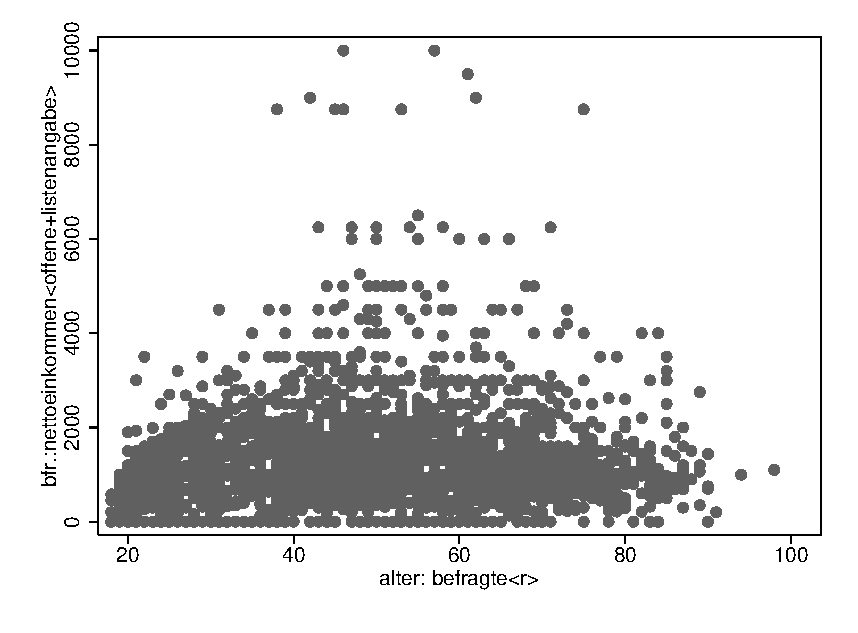
\includegraphics[width=8cm]{images/scatter.eps}}
\end{figure}
\end{frame}

\section{Boxplots}
\begin{frame}[fragile]{Boxplots} \index{Grafik!Boxplots} \index{Grafik!graph box}
\begin{lstlisting}
graph box hhinc
\end{lstlisting}
\begin{figure}
{\centering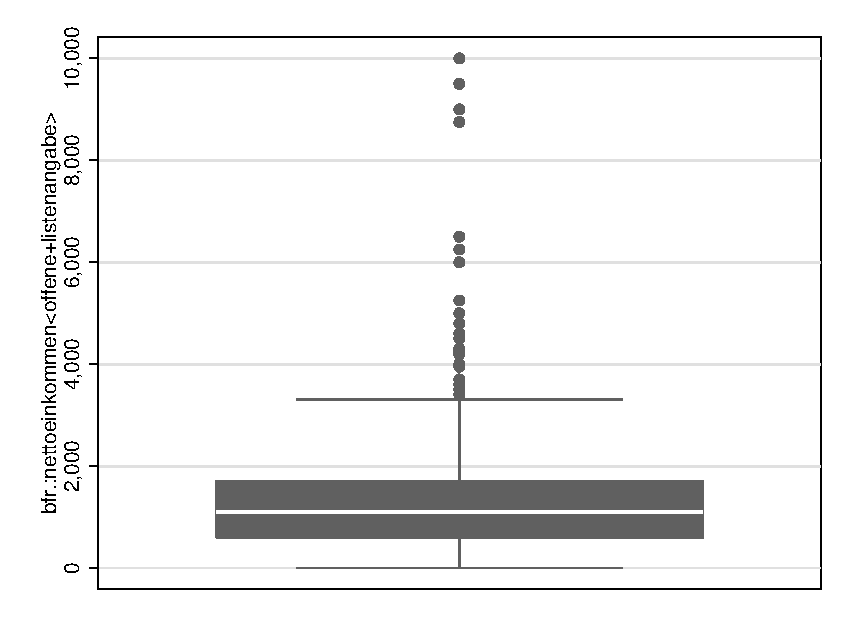
\includegraphics[width=8cm]{images/box.eps}}
\end{figure}
\end{frame}

\section{Histogramme}
\begin{frame}[fragile]{Histogramme} \index{Grafik!Histogramme} \index{Grafik!hist} \index{Grafik!hist freq}
\begin{lstlisting}
hist hhinc, freq
\end{lstlisting}
\begin{figure}
{\centering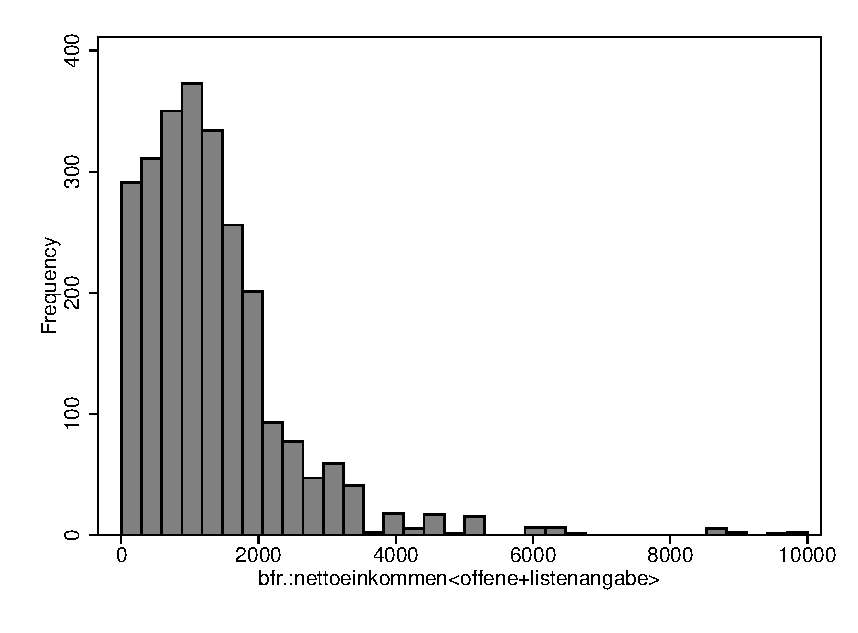
\includegraphics[width=8cm]{images/hist.eps}}
\end{figure}

  \begin{tikzpicture}[transform shape, rotate=10, overlay]
\node at (8,2) [mybox] (box) {%
    \begin{minipage}[t!]{0.35\textwidth}
    \tiny\textcolor{black}{\texttt{freq erzeugt Häufigkeiten, sonst steht auf der y-Achse die Dichte.}}
    \end{minipage}
    };
\end{tikzpicture}

\end{frame}

\section{Dot-Charts}
\begin{frame}[fragile]{Dot-Charts} \index{Grafik!Dot-Charts} \index{Grafik!graph dot} \index{Grafik! graph dot over()}
\begin{lstlisting}
graph dot (mean) hhinc, over(sex)
\end{lstlisting}
\begin{figure}
{\centering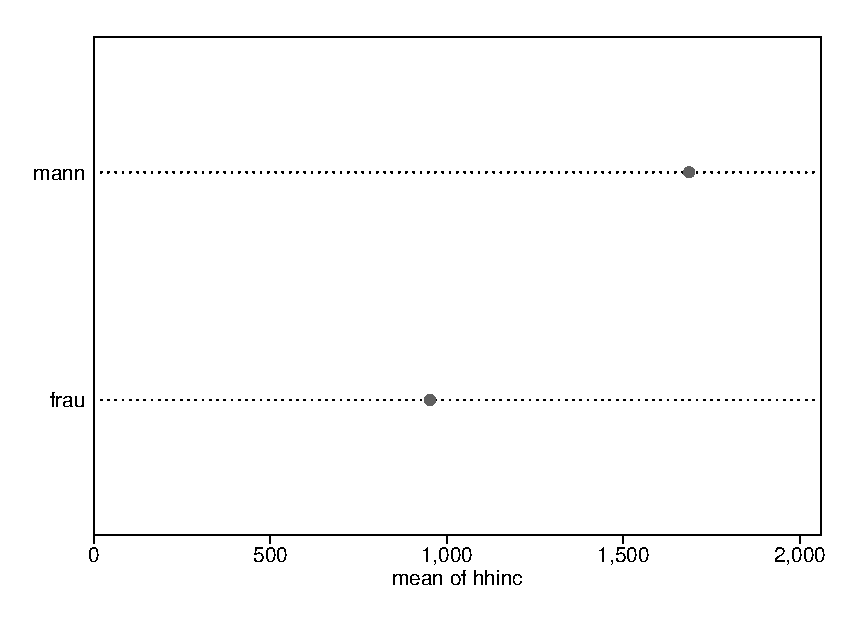
\includegraphics[width=8cm]{images/dot.eps}}
\end{figure}
\end{frame}


\section{Export von Grafiken}
\begin{frame}[fragile]{Export von Grafiken} \index{Grafik!exportieren}
\begin{lstlisting}
graph export "${OUTPUT}\graph1.pdf", replace
\end{lstlisting}
\begin{itemize}
\item Zum Export von Grafiken stehen mehrere Formate zur Verfügung
\item .ps .pes .wmf .emf .pdf .png .tif
\item Zur Weiterverarbeitung in MS-Office Programmen empfiehlt sich .png
\item Zur Weiterverarbeitung in TeX empfiehlt sich .pdf oder .eps
\end{itemize}
\end{frame}